\documentclass[a4paper]{article}

\usepackage[english]{babel}
\usepackage[utf8]{inputenc}
\usepackage{amsmath}
\usepackage{graphicx}
\usepackage[colorinlistoftodos]{todonotes}
%\usepackage[margin=0.6in]{geometry}
\usepackage{multirow}
\usepackage{subfig}
\usepackage[capposition=top]{floatrow}


\begin{document}

\begin{titlepage}
	\centering
	

\includegraphics[scale=0.5]{index.png}
	\vspace{1cm}
	
\newcommand{\HRule}{\rule{\linewidth}{0.5mm}} 

{\scshape\Large University of Witwatersrand\par}
{\scshape\Large Johannesburg, South Africa\par}
	\vspace{1.5cm}
	{\huge\bfseries Machine Learning Assignment \par}
	\vspace{2cm}
	{\Large\itshape Tamlin Love, Zachary Bowditch\par}
	\vspace{0.5cm}
	{\Large\itshape 1438243, 1414769\par}
	\vfill
	
\HRule \\[0.4cm]
{ \huge \bfseries Comparative Analysis of Machine Learning Methods on Chord Classification}\\[0.4cm] 
\HRule \\[1.5cm]

	{\large Semester 1, 2018\par}

\end{titlepage}
\section{Introduction}
The aim of this assignment is to use machine learning techniques (namely, a \textbf{Naïve Bayes Classifier} and an \textbf{Artificial Neural Network}) to classify musical chords. The problem is not as simple as it may first appear to be. Musical chords are defined by the pitches that occur within them (for example, a C Major chord is typically composed of $C$, $E$ and $G$), but additional pitches played during the event might obscure the chord. An example of such a pitch is a \textit{passing note}, which does not belong to chord in which it occurs but resolves to a chord-tone in the next chord. Chord notes can also be missing. For example, a chord composed of $C$ and $E$ resonates with the sound of C Major despite lacking the $G$. The issue is further complicated when more diverse chords, such as \textit{sixth chords} or \textit{ninth chords}, are added to the mix. We wish to investigate how well our chosen machine learning techniques perform in this classification, given these challenges.
\section{Dataset}
The dataset used is the \textbf{Bach Chorale Harmony Data Set} compiled by Daniele P. Radicioni and Roberto Esposito. The set consists of 5665 chords (or \textit{events}) from 60 chorales by J.S. Bach (1685 - 1750). Each chord is composed of the following attributes:
\begin{itemize}
\item Chorale ID: An ID identifying the chorale from which the chord is taken.
\item Event Number: An integer denoting the position of chord within the chorale
\item Pitch Class: 12 yes/no values denoting whether or not a given pitch is in the chord. Ordered $C$,$C\sharp$,$D$,$D\sharp$, etc. until $B$.
\item Bass: The bass (lowest) note of the chord
\item Meter: Integer from 1 to 5, denoting how accented the chord is. Lower numbers indicate less accenting, higher numbers indicate more accenting
\end{itemize}
Each event is also assigned a chord, which is the target for this classification problem. The following image shows a few of the entries within the dataset.
\begin{figure}[h]
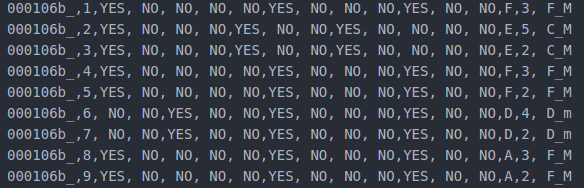
\includegraphics[scale=0.5]{BachChoraleDatasetExample.png}
\caption{Example dataset entries}
\end{figure}
%\pagebreak
\section{Data Processing}
Fortunately, the dataset is well structured and required no cleaning. However, one potential problem present in the data that we addressed is the issue of \textit{enharmonic equivalents}: that is, notes that have the same pitch but are labelled differently depending on context. For example, $D\sharp$ and $E\flat$ sound the same, yet one would never find an $E\flat$ in a B Major chord, instead finding a $D\sharp$. 
\\[12pt]
In the dataset, the pitch class attributes (the pitches appearing in the event) are labelled using enharmonic equivalents. Thus $D\sharp$ and $E\flat$ are considered identical, for example. However, the bass note attribute and the chord label target are not labelled using enharmonic equivalents. Thus, for example, a $D\sharp$ in the bass is considered different from an $E\flat$, and similarly D$\sharp$ Major and E$\flat$ Major are treated as different classes.
\\[12pt]
To address this problem, we can treat enharmonic equivalents as identical. This approach has the added effect of reducing the number of chord classes from 102 to 93, which should effect accuracy. We compare our accuracy with and without this approach in later sections.
\\[12pt]
The data structures used to represent the data differ across the programs.
\\[12pt]
For the Naïve Bayes Classifier, each of the target chords was represented as a Python dictionary and the occurence of every attribute (12 chord pitches, 12 bass note pitches, 5 meters) was represented as a key within said dictionary.
The Neural Network imported the data similarly, representing each data point in the form of a 1D vector comprising 1s and 0s, which each value indicating the presence or absence of a particular feature (see section 4.2 for a more detailed description).
\\[12pt]
For the Naïve Bayes Classifier, the data was split with 80\% of the data used in training and 20\% used in testing. The Neural Network randomly divides the data into the training set (60\%), the testing set (20\%) and the validation set (20\%).
\section{Learning Methods}
\subsection{Naïve Bayes Classifier}
The first of our programs implements a Naïve Bayes classifier with Laplace smoothing. It is a good method to implement as it is fast to run, simple to implement and tends to perform well with categorical, "bag of words" inputs. It does assume conditional independence however, which does not reflect reality and thus may result in lower accuracy. Overall, the method gives us a good baseline with which to compare other methods. The Python code can be found in the \textit{NaiveBach.py} file, with helper functions in the \textit{BachControl.py} file. 
\\[12pt]
In the \textit{NaiveBach.py} file, feature inclusion and the use of enharmonic equivalents are controlled by boolean variables. The program first reads in the data and processes it into the dictionaries described in the previous section. The data is randomly segmented into training and testing sets. During learning, it counts the occurence of each attribute for each target chord and the, during testing, applies the Bayesian probability formula (assuming conditional independence) for each target class to obtain probabilities for every chord. It then classifies the data by choosing the chord with the highest probability. This is repeated 50 times to produce an average confusion matrix and lessen the potential impact of the random partitioning of the dataset into training and testing sets.
\\[12pt]
Laplace smoothing was employed, with values $k=1$ and $n^{k}=2$ (as each attribute has two possible values, either a 1 marking presence or 0 marking absence). 
\\[12pt]
Unfortunately, due to the high number of classes in the dataset, the confusion matrices for the method cannot be included within this document. They can be found attached with the code.
\\[12pt]
When run with all features included and without the use of enharmonic equivalents, the program has an average accuracy of $68.93\%$ (see \textit{NB\textunderscore confusion\textunderscore 1}). This is quite a good result, considering that the method relies on the false assumption of conditional independence between notes in a chord, and that the program in no way takes into account the context (i.e. neighbouring chords) around a particular chord.
\\[12pt]
When run with the use of enharmonic equivalents, the accuracy of the program increases slightly to $69.08\%$ (see \textit{NB\textunderscore confusion\textunderscore 2}). This is expected as the distribution of chords indicates that Bach preferred using certain enharmonic equivalents to others (e.g. E$\flat$ Major appears 146 times while D$\sharp$ Major appears twice), and thus there are not enough occurrences of enharmonically equivalent chords for there to be a significant increase in accuracy.
\\[12pt]
We also examine the contribution of each of the features towards accuracy. When chord notes are not used (i.e. only bass note and meter are taken into account) with the use of enharmonic equivalents, accuracy drops to $33.61\%$ (see \textit{NB\textunderscore confusion\textunderscore 3}). This is expected, as the notes within a chord define what the chord is, and are necessary for correct classification for the chord. In fact, this accuracy is higher than expected (it is, after all, better than random guessing). When bass notes are not used, accuracy drops slightly to $67.65\%$ (see \textit{NB\textunderscore confusion\textunderscore 4}), indicating that, while bass notes contribute to the classification of a chord, they do not contribute much. 
\\[12pt]
Finally, when meter is not used, accuracy actually improves slightly to $69.98\%$ (see \textit{NB\textunderscore confusion\textunderscore 5}), indicating that the feature is actually slightly obfusticating the classification. The reasoning behind this feature is that more stable chords (simple major or minor chords, for example) would be accented more than less stable chords (diminished or fourth chords, for example). However, our results indicate this may not be the case.
\\[12pt]
Across all tests, the most common errors in classification tend to be a "simplification" of certain chords. For example, C Dominant 7th chords (composed of $C$, $E$, $G$ and $B\flat$) are frequently mistaken for C Major chords (composed of just $C$, $E$, $G$). The former can be seen as an extension of the latter and has many of the same qualities and functions. It is a common error in beginner music students and thus it makes sense for these errors to occur here. Unfortunately, these errors are a symptom of the assumption of conditional independence, and thus cannot be properly addressed in the context of a Naïve Bayes Classifier.
\\[12pt]
Overall, little improvement in accuracy beyond our initial test is made when including or excluding features or when altering the dataset to make use of enharmonic equivalents. This is likely due to a number of factors, including the aformentioned assumption of conditional independence and the fact that neighbouring chords (which provide musical context) are not considered. Additionally, the chords are distributed very unevenly and thus the algorithm tends to favour more frequently occuring chords to those that appear very infrequently. There is also a high chance that certain chords never appear in the training set and thus cannot ever be predicted. Certain techniques, such as oversampling or cost-sensitive learning, may be used to correct for this.
\subsection{Artificial Neural Network}
The choice of making use of this machine learning technique, a feed-forward artificial neural network, was largely inspired by the enticing scent of the aura encompassing the universal explosion of Deep Learning. Its applications are vast and flexible. From MNIST digit classification to claiming 1st place as the quickest and strongest chess playing architecture the world has seen so far, Deep Learning has proved to be the most versatile and impactful learning technique in many areas in AI.
\\[12pt]
The choice of the language with which to implement the neural network was C++, in order to better understand the underlying functionality of neural network mechanics. Although slower than more optimized linear algebra libraries, such as Numpy in Python, our implementation thankfully executed slightly faster than was anticipated. The code can be examined in "ann.cpp" and can be run with the already compiled executable, "ann", whose run instructions are delineated in the "README.txt" file.
\\[12pt]
The architecture of the ANN is shown, scaled down for neatness, in Figure 2 below.
\\[12pt]
\begin{figure}[h]
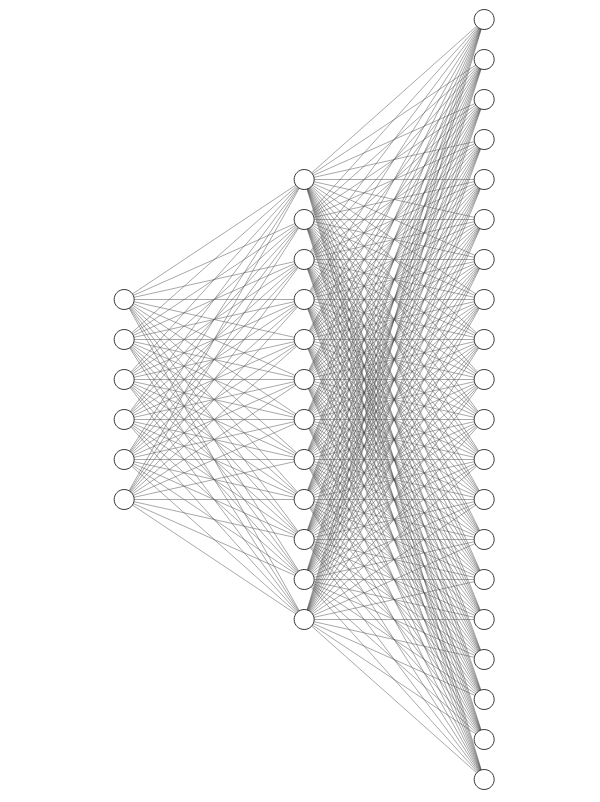
\includegraphics[scale=0.2]{neuralnet.png}
\caption{Scaled down visual representation of the ANN}
\end{figure}
The first layer has 29 input neurons (whose format will be addressed later on), the one hidden layer comprises 60 neurons, and the last (output) layer contains 102 layers, with each neuron representing a class, or in this specific exercise, a chord. 
\\[12pt]
To predict the chord from the input notes, the network will tweak its weights and biases using an online learning algorithm through which the parameter updates are made after each item in the training set is propagated through the network.
\\[12pt]
The means by which these updates are made is the back propagation algorithm, which estimates the errors made by each neuron and tweaks them accordingly, minimizing a cost function (in this case, the quadratic cost function sufficed. See figure (3)). In order for back propagation to estimate the aforementioned errors, there is needed a comparison between the networks predicted chord class and the actual class of each of the inputs within the training set. For each item in the training set, the ANN's first layer is set to the 29 input values and each subsequent neuron applies weights (which are randomized between 0 and 1 to start with) to the values it receives, sums them, and then adds a bias (initial value = 1). Finally, the neuron \textit{activates} by applying the convenient sigmoid function (denoted by $\sigma$ below) to the summation described above:
\begin{eqnarray}
z = \sum_i{w_ia_i} + b
\end{eqnarray}
\begin{eqnarray}
\sigma(z) = \frac{1}{1 + e^{-z}}
\end{eqnarray}
Expression (1) is executed for each neuron in the network, meaning that for out particular network, this computation is made 60 + 102 = 162 times. The sigmoid function (2) maps the z value to a point between 0 and 1, exactly the range we need to classify the data. When the output is calculated, the value closest to 1 is taken to be the index of the predicted class.
\\[12pt]
The input vector of 29 indices is constructed as follows:
The first 12 indices are marked 0 or 1, with 1 indicating the presence of a note in the chord. The next 12 indices are all marked 0 except for one which is marked 1 to indicate the bass note (out of the same 12 pitches). The next 5 are also marked 0 except for one which is marked 1 to indicate one of 5 possible meters (whose function in the input is described in \textit{Dataset}).
\\[12pt]
As was mentioned previously, the cost function used was the quadratic cost function as shown below, where $v_i$ is the classification vector representing the network's predicted chord:
\begin{eqnarray}
\frac{1}{2}\sum_{i = 1}^n{(y_i - v_i)^2}
\end{eqnarray}
To test this design, the focus was to predict each chord \textbf{without} merging enharmonic equivalents (without treating them as the same note). (see \textit{Data Processing}), to see how well the network could "understand" pitch. Initially, only training and testing sets were used, by randomly dividing the dataset into two subsets with the training set making up 80\% and the testing set, the remaining 20\%. An accuracy of approximately 72\% was obtained consistently over many cycles of execution (where one cycle is the training algorithm working up to a number of epochs), each restricted to 1000 epochs. However, in order to determine whether or not the network could examine and extrapolate unseen data, the choice was made to generate a third subset of the data, the validation set, with which we could test-drive the network as it stood after a constant number of epochs. With a learning rate of -0.1 (chosen so that a slow descent could occur, with gradual adjustments being made to each of the the network's parameters), the network's improvement quickly capped around 70\% after about 150 epochs, making only fractional adjustments up and down.
\\[12pt]
To obtain the accuracy of the predictions made on the validation data, an average of five cycles was taken (see below) for both the regularized and non-regularized training algorithm. The following scatter plot of the third cycle of non-regularized training process, typifies the behavior of the test data accuracy's improvement seen across all of the cycles:
\\[12pt]
\begin{figure}[h]
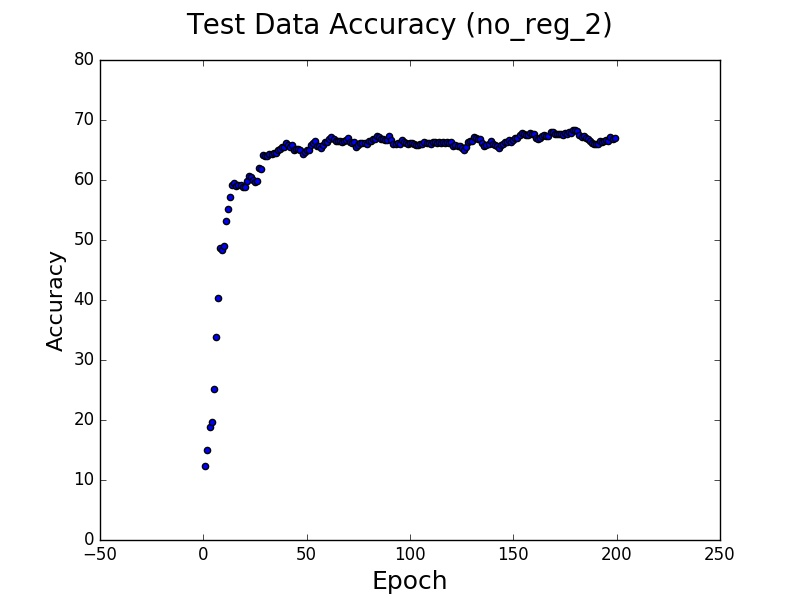
\includegraphics[scale=0.2]{no_reg_2.jpg}
\caption{Accuracy of test data against the number of epochs. Learning Rate = -0.1}
\end{figure}

As can be clearly seen, the accuracy very quickly plateaus around 67\%, a somewhat disappointing figure. However, this is insightful in that the network appears to exhibit a similarly degree of accuracy in prediction as the Naïve Bayes classifier, as discussed previously, for what one could assume to be the same reasons as those stated in section 4.1. The same plateau occurs for higher and lower learning rates, just at different epochs. The other scatter plots, generated by "graph\textunderscore network\textunderscore performance.py", coupled with their respective data files, can be found in the "Artificial Neural Network" folder in this directory.

\begin{figure}[h]
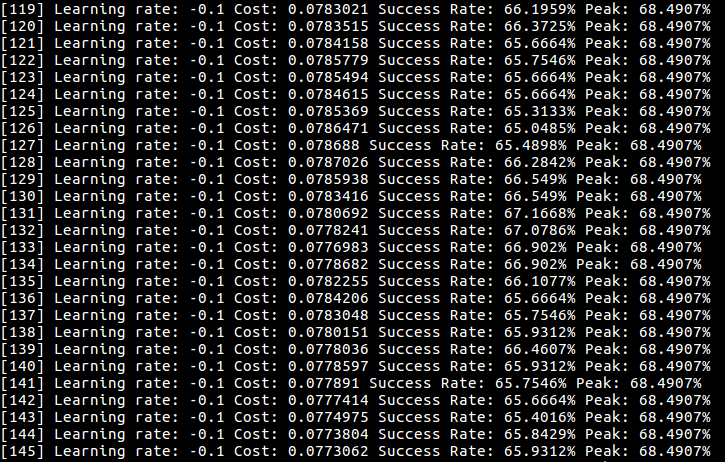
\includegraphics[scale=0.3]{learning.png}
\caption{The learning process.}
\end{figure}
\pagebreak
On the validation set the following accuracies were obtained:
\\\\
Validation Set Accuracy [after 200 epochs] [No regularization] [Average of five executions]: 66.549\%\\\\
Validation Set Accuracy [after 200 epochs] [Regularization] [Average of five executions]: 65.5605\%\\

As the accuracies of the regularized and the non-regularized parameters only differ by approximately 1\%, it can be observed that the regularization has minimal effect on the classification. Many layer configurations were tested, each performing to the same degree of accuracy or less. Perhaps with a more extensive examination of layer architecture, a more reliable network could be constructed.

\section{Results and Conclusion}
In comparing the two techniques, we find that both the \textbf{Naïve Bayes Classifier} and the \textbf{Artificial Neural Network} produce similar results. This indicates that the use of various machine learning methods is unlikely to result in consistently higher accuracy. We hypothesize that a larger, more evenly distributed dataset would produce somewhat improved results. We also believe that altering the learning algorithm to keep track of the context of a chord (i.e. the chords before and after the chord in question) would improve accuracy.



\section{References}
\subsection{Dataset}
https://archive.ics.uci.edu/ml/datasets/Bach+Choral+Harmony
\subsection{Neural Network}
http://neuralnetworksanddeeplearning.com/ (Michael Neilsen)\\
http://alexlenail.me/NN-SVG/index.html (Neural Network diagram)
\end{document}